
\section{Пример: данные по гормонам}
Давайте снова посмотрим на пример данных по гормонам из 9 главы. Для удобства повторно изобразим данные на рисунке 17.1. Напомним, что переменная отклика $y_{i}$ --- это количество противовоспалительного гормона, оставшегося в устройстве после $z_{i}$ часов его ношения. Устройства были случайным образом выбраны из трех партий $A, B$ и $C$, которые обозначены буквами на графике.
\begin{figure}[h]
\center{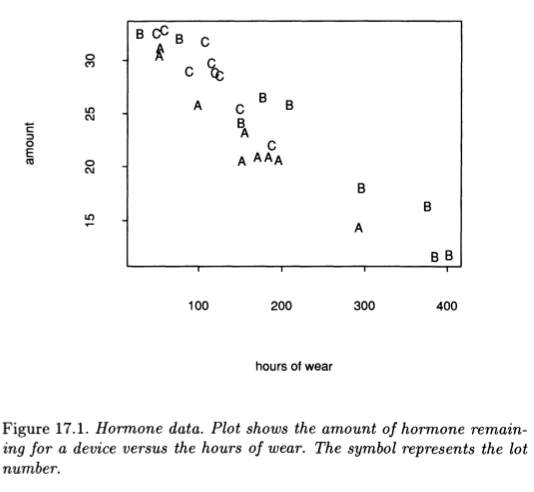
\includegraphics[width=1 \linewidth]{17/f17.1.png}}
\end{figure}
В девятой главе мы строили модель регрессии по данным каждой партии с разными свободными, но одинаковыми угловыми коэффициентами. Оценки приведены в таблице 9.3 на 110 странице.

Здесь мы обсудим два вопроса: 1) Насколько хорошо модель предсказывает количество оставшегося гормона для нового устройства? 2) Прогнозирует ли эта модель лучше (или хуже), в случае, когда у нас одна линия регрессии? Чтобы ответить на первый вопрос, мы могли бы посмотреть на среднюю остаточную ошибку по всем $n = 27$ наблюдениям,
\begin{equation}
\frac{\tx{RSE}}{n} = \summ{1}{n} \frac{(y_{i} - \what{y_{i}})^{2}}{n} = 2.20,
\end{equation}
но это может быть слишком <<оптимистично>>, и истинная ошибка педсказания, возможно, будет недооценена. Дело в том, что мы используем для оценки модели те же данные, что и для ее обучения, используя оценки параметров, которые подобраны на этом же наборе данных. Другими словами, тестовая выборка, иногда называемая обучающей выборкой, такая же, как и исходная. Полученные таким образом оценки для ошибок предсказания называют видимыми ошибками.

Способ исправить $(17.3)$ --- это заменить деление на $n$ на деление на $n - p$, где $p$ --- количество признаков. Это помогает сделать обычную оценку остаточной дисперсии несмещенной $\what{\sigma}^{2} = \summ{}{}  \frac{(y_{i} - \what{y_{i}})^{2}}{n- p}$. Мы увидим, что для решения проблемы необходимы более серьезные исправления.